\begin{figure}[h]
  \centering
  \subfloat[]{
  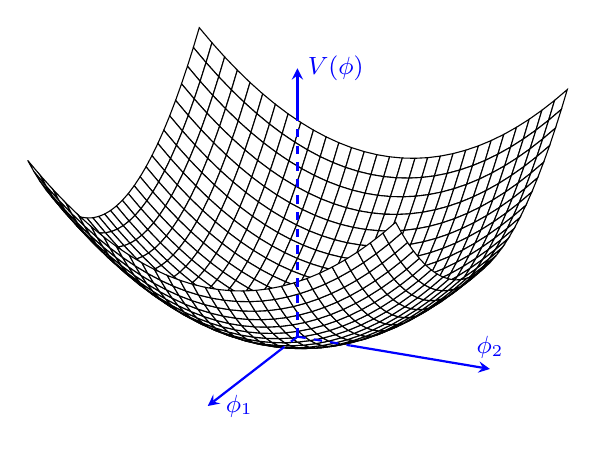
\begin{tikzpicture}%[scale=0.85]
    \begin{axis}[
        hide axis,
        %axis lines=middle,
        %            axis on top,
        %            axis line style={blue,dashed,thick},
        %            ymin=-2,ymax=2,
        %            xmin=-2,xmax=2,
        %            zmin=-2,zmax=2,
        samples=30,
        domain=-0.9:0.9,
        y domain=-0.9:0.9,clip=false
      ]
      \addplot3 [surf, shader=flat, draw=black, fill=white, z buffer=sort]
      ({0.85*x},{0.85*y},{0.85*x^2+y^2});
      \draw[blue,thick,dashed] (axis cs:0,0,0) -- (axis cs:0.22,0,0);
      %node[below,font=\small]{$\phi_{\text{IM}}$};
      \draw[blue,thick,-stealth] (axis cs:0.22,0,0) -- (axis cs:0.8,0,0)
      node[above,font=\small]{$\phi_{2}$};
      \draw[blue,thick,dashed] (axis cs:0,0,0) -- (axis cs:0,-0.15,0);
      %node[left=2mm,font=\small]{$\phi_{\text{RE}}$};
      \draw[blue,thick,-stealth] (axis cs:0,-0.15,0) -- (axis cs:0,-0.8,0)
      node[right=1mm,font=\small]{$\phi_{1}$};
      \draw[blue,thick,dashed] (axis cs:0,0,0) -- (axis cs:0,0,1.55);
      \draw[blue,thick,-stealth] (axis cs:0,0,1.55) -- (axis cs:0,0,1.9)
      node[right,font=\small]{$V(\phi)$};
    \end{axis}
  \end{tikzpicture}}
  \hspace{15mm}
  \subfloat[]{
  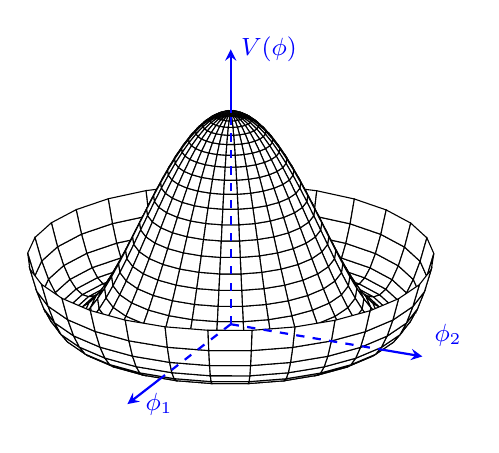
\begin{tikzpicture}
    \begin{axis}[
        hide axis,
        %axis lines=middle,
        %            axis on top,
        %            axis line style={blue,dashed,thick},
        %            ymin=-2,ymax=2,
        %            xmin=-2,xmax=2,
        %            zmin=-2,zmax=2,
        samples=30,
        domain=0:360,
        y domain=0:1.25,clip=false
      ]
      \addplot3 [surf, shader=flat, draw=black, fill=white, z buffer=sort]
      ({sin(x)*y}, {cos(x)*y}, {(y^2-1)^2});
      \draw[blue,thick,dashed] (axis cs:0,0,0) -- (axis cs:1,0,0);
      %node[below,font=\small]{$\phi_{\text{IM}}$};
      \draw[blue,thick,-stealth] (axis cs:1,0,0) -- (axis cs:1.3,0,0)
      node[above,font=\small]{~~~~~~$\phi_{2}$};
      \draw[blue,thick,dashed] (axis cs:0,0,0) -- (axis cs:0,-1,0);
      %node[left=2mm,font=\small]{$\phi_{\text{RE}}$};
      \draw[blue,thick,-stealth] (axis cs:0,-1,0) -- (axis cs:0,-1.5,0)
      node[right=1mm,font=\small]{$\phi_{1}$};
      \draw[blue,thick,dashed] (axis cs:0,0,0) -- (axis cs:0,0,1)
      %node[left=2mm,font=\small]{$\phi_{\text{RE}}$}
      ;
      \draw[blue,thick,-stealth] (axis cs:0,0,1) -- (axis cs:0,0,1.3)
      node[right,font=\small]{$V(\phi)$};
    \end{axis}
  \end{tikzpicture}}
  \caption{The Higgs potential in its fully and broken symmetric forms.}
  \label{fig:higgs-pot-01}
\end{figure}
